%!TEX encoding = UTF-8 Unicode
%!TEX root = ../lect-week02.tex

%\Subsection{Samlingar och loopar}
\Subsection{Datastrukturer och kontrollstrukturer}


\begin{Slide}{Vad är en datastruktur?}\SlideFontSmall
\begin{itemize}
\item En \href{https://sv.wikipedia.org/wiki/Datastruktur}{datastruktur} är en struktur för organisering av data som...
\begin{itemize}\SlideFontTiny
\item kan innehålla \Alert{många} element,
\item kan refereras till med \Alert{ett} enda namn, och
\item ger möjlighet att komma åt de enskilda elementen.
\end{itemize}

\item En \Emph{samling} \Eng{collection} är en datastruktur som kan innehålla många element av \Alert{samma typ}.

\item Exempel på olika samlingar där elementen är organiserade på olika vis: \\ 
\vspace{0.5em}
\begin{tabular}{l c}
\Emph{Lista} & 
\includegraphics[width=5cm]{../img/list.pdf} \\
\Emph{Träd}  & 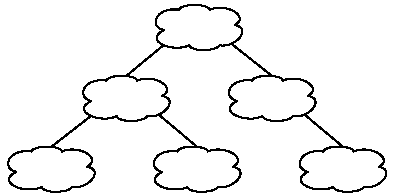
\includegraphics[width=2.2cm]{../img/tree.pdf} \\
\Emph{Graf}  & 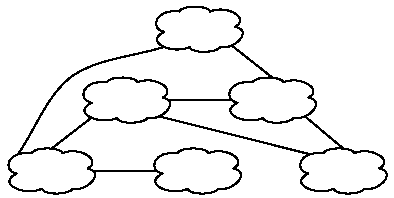
\includegraphics[width=2.2cm]{../img/graph.pdf} \\
\end{tabular}
\end{itemize}
{
\SlideFontTiny \vspace{1em }\hskip2em
Mer om listor \& träd \href{http://cs.lth.se/edaa01vt}{fördjupningskursen}. 
Mer om träd, grafer i \href{http://cs.lth.se/edaa40}{Diskreta strukturer.}
}

\end{Slide} 


\begin{Slide}{Vad är en vektor?}\SlideFontSmall
En \Emph{vektor}\footnote{Vektor kallas ibland på svenska även \href{https://sv.wikipedia.org/wiki/F\%C3\%A4lt_\%28datastruktur\%29}{fält}, men det skapar stor förvirring eftersom det engelska ordet \emph{field} ofta används för \emph{attribut} (förklaras senare).} 
\Eng{vector, \href{https://en.wikipedia.org/wiki/Array_data_structure}{array}} är en \Emph{samling} som är \Alert{snabb} att \Emph{indexera} i. 
Åtkomst av element sker med \code{apply(platsnummer)}: 

\begin{REPL}
scala> val heltal = Vector(42, 13, -1, 0 , 1)
heltal: scala.collection.immutable.Vector[Int] = Vector(42, 13, -1, 0, 1)

scala> heltal.apply(0)
res0: Int = 42

scala> heltal(1)    // man kan skippa .apply
res1: Int = 13

scala> heltal(5)
java.lang.IndexOutOfBoundsException: 5
  at scala.collection.immutable.Vector.checkRangeConvert(Vector.scala:132)
\end{REPL}
Utelämnar du \code{.apply} så gör kompilatorn anrop av \code{apply} ändå om det går.
\end{Slide}

\begin{Slide}{En konceptuell bild av en vektor}

\begin{REPLnonum}
scala> val heltal = Vector(42, 13, -1, 0 , 1)

scala> heltal(0)
res0: Int = 42
\end{REPLnonum}

\begin{tikzpicture}[font=\ttfamily]
\matrix [matrix of nodes, row sep=0, column 2/.style={nodes={rectangle,draw,minimum width=3em}}] (var) at (0cm, 2.8cm)
{
heltal   &  \makebox(16,12){ }\\
};
\matrix [matrix of nodes, draw=black,row sep=0, column 2/.style={nodes={rectangle,draw,minimum width=4em}}] (vec) at (4cm, 1cm)
{
\textit{plats} &  \\
0   &  \makebox(16,12){42}\\
1   &  \makebox(16,12){13}\\
2   &  \makebox(16,12){-1}\\
3   &  \makebox(16,12){0}\\
4   &  \makebox(16,12){1}\\
};
\filldraw[black] (0.7cm,2.8cm) circle (3pt) node[] (ref) {};
 \draw [arrow] (ref) -- (vec);
\end{tikzpicture}

%\vspace{1em} Elementen ligger på rad någonstans i minnet.
\end{Slide}



\begin{Slide}{En samling strängar}

\begin{itemize}
\item En vektor kan lagra många värden av samma typ. 
\item Elementen kan vara till exempel heltal eller strängar. 
\item Eller faktiskt vad som helst. 
\end{itemize}

\begin{REPL}
scala> val grönsaker = Vector("gurka","tomat","paprika","selleri")
grönsaker: scala.collection.immutable.Vector[String] = Vector(gurka, tomat, paprika, selleri)

scala> val g = grönsaker(1)
g: String = tomat

scala> val xs = Vector(42, "gurka", true, 42.0)
xs: scala.collection.immutable.Vector[Any] = Vector(42, gurka, true, 42.0)


\end{REPL}

\end{Slide}

\begin{Slide}{Vad är en kontrollstruktur?}
\begin{itemize}
\item En \Emph{kontrollstruktur} påverkar \Alert{sekvensen}.
\begin{itemize}
\item[] Exempel på inbyggda kontrollstrukturer: 
\\\vspace{0.5em}\code{for}-sats, \code{while}-sats
\end{itemize}

\item[]

\item I Scala kan man definiera \Emph{egna} kontrollstrukturer.
\begin{itemize}
\item[] Exempel: \code{upprepa} som du använt i Kojo
\\\vspace{0.5em}\code|upprepa(4){fram; höger}|
\end{itemize}
\end{itemize}
\end{Slide}


\begin{Slide}{Mitt första program: en oändlig loop på ABC80}
\begin{columns}
\begin{column}{0.8\textwidth}
\begin{verbatim}
10 print "hej"
20 goto 10
\end{verbatim}
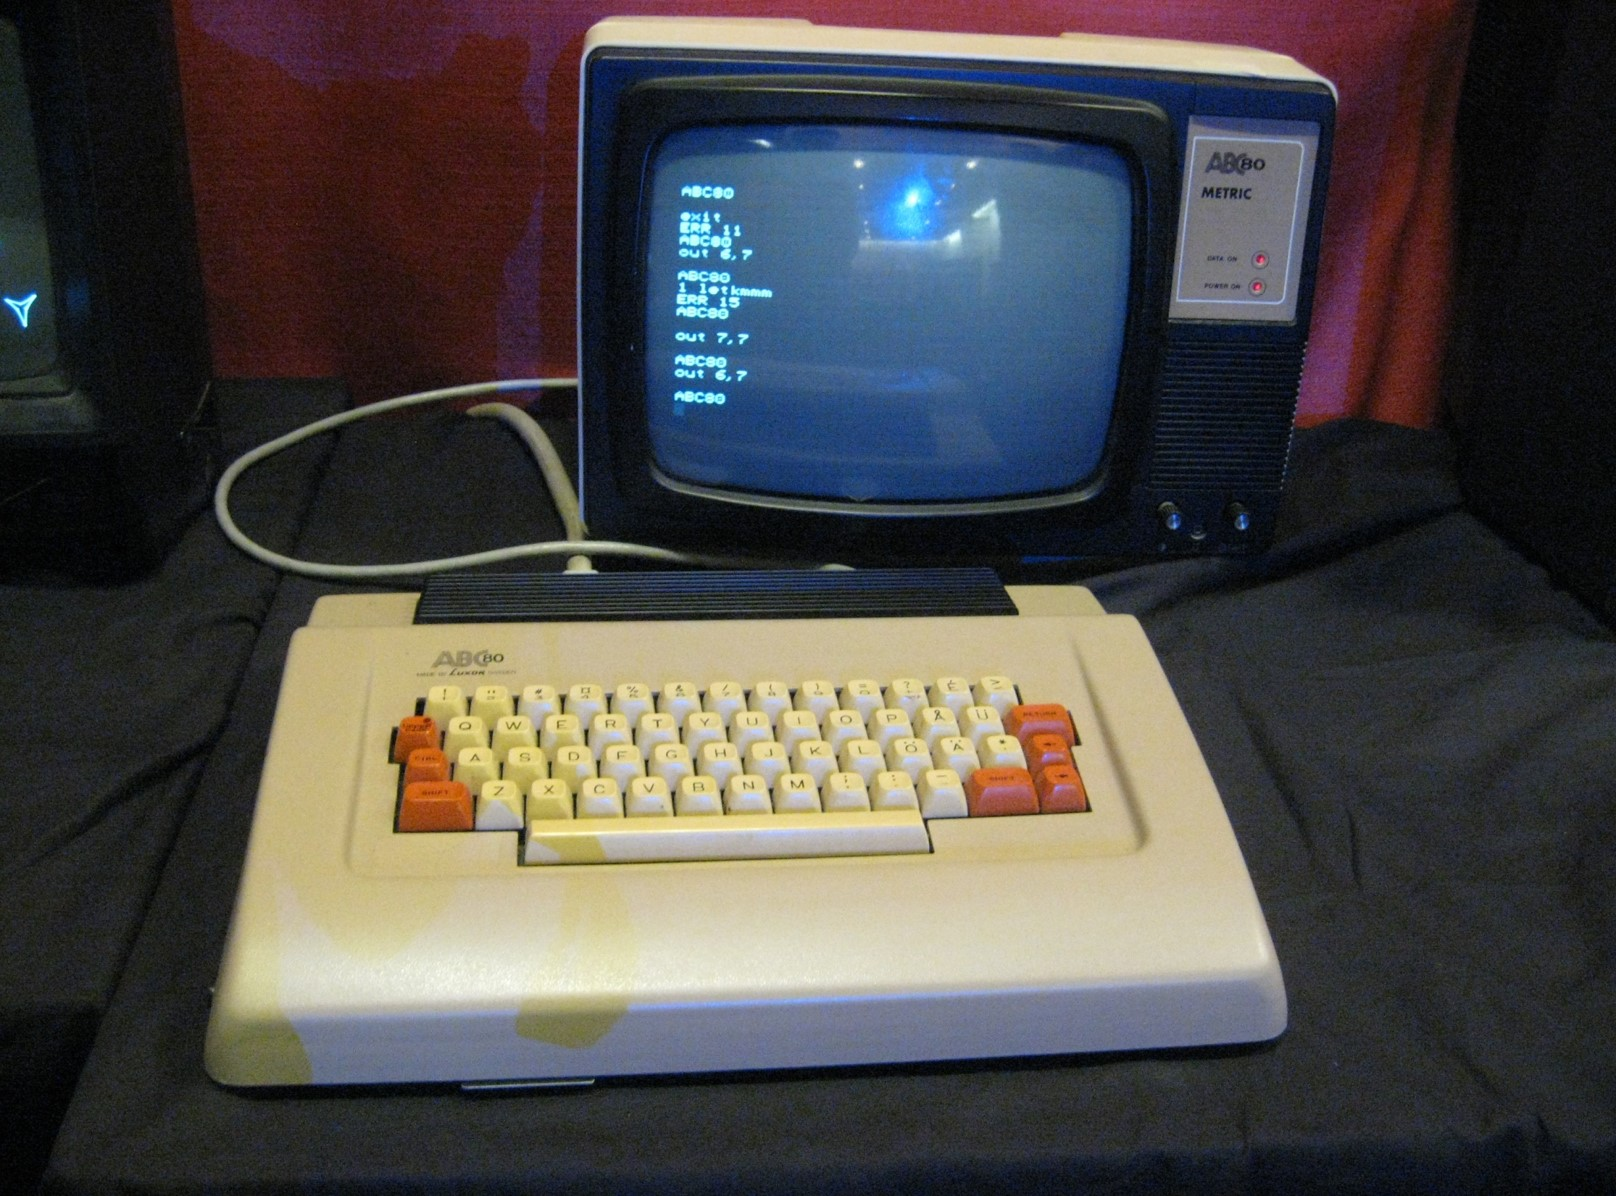
\includegraphics[width=0.8\textwidth]{../img/abc80.jpg}
\end{column}
\begin{column}{0.3\textwidth}
\pause
\begin{verbatim}
hej
hej
hej
hej
hej
hej
hej
hej
hej
hej
hej
hej
<Ctrl+C>
\end{verbatim}

\end{column}
\end{columns}
\end{Slide}


\begin{Slide}{Loopa genom elementen i en vektor}
En \code{for}-\Emph{sats} som skriver ut alla element i en vektor:
\begin{REPL}
scala> val grönsaker = Vector("gurka","tomat","paprika","selleri")

scala> for (g <- grönsaker) println(g)
gurka
tomat
paprika
selleri

\end{REPL}

\end{Slide}


\begin{Slide}{Bygga en ny samling från en befintlig med for-uttryck}
Ett \code{for}-\code{yield}-\Emph{uttryck} som \Emph{skapar en \Alert{ny} samling}.

\begin{Code}[basicstyle=\ttfamily\fontsize{12}{14}\selectfont]
for (g <- grönsaker) yield "god " + g
\end{Code}

\begin{REPL}
scala> val grönsaker = Vector("gurka","tomat","paprika","selleri")

scala> for (g <- grönsaker) yield "god " + g
res0: scala.collection.immutable.Vector[String] = 
  Vector(god gurka, god tomat, god paprika, god selleri)

scala> val åsikter = for (g <- grönsaker) yield s"god $g"
åsikter: scala.collection.immutable.Vector[String] = 
  Vector(god gurka, god tomat, god paprika, god selleri)
\end{REPL}

\end{Slide}


\begin{Slide}{Samlingen \code{Range} håller reda på intervall}
\begin{itemize}
\item Med en \code{Range(start, slut)} kan du skapa ett intervall: \\ från och med \code{start} till (men inte med) \code{slut}
\end{itemize}

\begin{REPLnonum}
scala> Range(0, 42)
res0: scala.collection.immutable.Range = 
  Range(0, 1, 2, 3, 4, 5, 6, 7, 8, 9, 10, 11, 12, 13, 14, 
    15, 16, 17, 18, 19, 20, 21, 22, 23, 24, 25, 26, 27, 28, 
    29, 30, 31, 32, 33, 34, 35, 36, 37, 38, 39, 40, 41)
\end{REPLnonum}

\begin{itemize}
\item Men alla värden däremellan skapas inte förrän de behövs:
\end{itemize}

\begin{REPL}
scala> val jättestortIntervall = Range(0, Int.MaxValue)
jättestortIntervall: scala.collection.immutable.Range = Range(0, 1, 2, 3, 4, 5, ...

scala> jättestortIntervall.end
res1: Int = 2147483647

scala> jättestortIntervall.toVector
java.lang.OutOfMemoryError: GC overhead limit exceeded
\end{REPL}

\end{Slide}

\begin{Slide}{Loopa med Range}
\code{Range} används i for-lopar för att hålla reda på antalet rundor.
\begin{REPLnonum}
scala> for (i <- Range(0, 6)) print(" gurka " + i)
 gurka 0 gurka 1 gurka 2 gurka 3 gurka 4 gurka 5 
\end{REPLnonum}
Du kan skapa en \code{Range} med \code{until} efter ett heltal:
\begin{REPLnonum}
scala> 1 until 7
res1: scala.collection.immutable.Range = 
  Range(1, 2, 3, 4, 5, 6)

scala> for (i <- 1 until 7) print(" tomat " + i) 
 tomat 1 tomat 2 tomat 3 tomat 4 tomat 5 tomat 6

\end{REPLnonum}
\end{Slide}

\begin{Slide}{Loopa med Range skapad med \texttt{to}}

Med \code{to} efter ett heltal får du en \code{Range} till och \Emph{med} sista:
\begin{REPLnonum}
scala> 1 to 6
res2: scala.collection.immutable.Range.Inclusive = 
  Range(1, 2, 3, 4, 5, 6)

scala> for (i <- 1 to 6) print(" gurka " + i) 
 gurka 1 gurka 2 gurka 3 gurka 4 gurka 5 gurka 6
 
\end{REPLnonum}


\end{Slide}



\begin{Slide}{Vad är en \code{Array} i JVM?}


\begin{itemize}
\item En \code{Array} liknar en \code{Vector} men har en särställning i JVM:
\begin{itemize}
\item Lagras som en sekvens i minnet på efterföljande adresser.
\item \Emph{Fördel}: snabbaste samlingen för element-access i JVM.
\item Men det finns en hel del \Alert{nackdelar} som vi ska se senare.
\end{itemize}

\end{itemize}

\begin{REPLnonum}
scala> val heltal = Array(42, 13, -1, 0 , 1)
\end{REPLnonum}

\begin{tikzpicture}[font=\ttfamily,scale=0.75, every node/.style={scale=0.75}]
\matrix [matrix of nodes, row sep=0, column 2/.style={nodes={rectangle,draw,minimum width=3em}}] (var) at (0cm, 2.8cm)
{
heltal   &  \makebox(16,12){ }\\
};
\matrix [matrix of nodes, draw=black,row sep=0, column 2/.style={nodes={rectangle,draw,minimum width=4em}}] (vec) at (4cm, 1cm)
{
\textit{plats} &  \\
0   &  \makebox(16,12){42}\\
1   &  \makebox(16,12){13}\\
2   &  \makebox(16,12){-1}\\
3   &  \makebox(16,12){0}\\
4   &  \makebox(16,12){1}\\
};
\filldraw[black] (0.7cm,2.8cm) circle (3pt) node[] (ref) {};
 \draw [arrow] (ref) -- (vec);
\end{tikzpicture}
\end{Slide}

\begin{Slide}{Några likheter \& skillnader mellan \texttt{Vector} och \texttt{Array}}\SlideFontSmall
\begin{multicols}{2}
\begin{REPL}[numbers=none]
scala> val xs = Vector(1,2,3)
\end{REPL}

\columnbreak

\begin{REPL}[numbers=none]
scala> val xs = Array(1,2,3)
\end{REPL}
\end{multicols}


Några likheter mellan \texttt{Vector} och \texttt{Array}
\begin{itemize}
\item Båda är samlingar som kan innehålla många element.

\item Med båda kan man snabbt accessa vilket element som helst: \code{xs(2)}

\item Båda har en fix storlek efter allokering.
\end{itemize}

Några viktiga skillnader:
\begin{multicols}{2}
\Emph{Vector}
\begin{itemize}
\item Är \Emph{oföränderlig}: du kan lita på att elementreferenserna aldrig någonsin kommer att ändras.

\item Är \Emph{snabb på att skapa en delvis förändrad kopia}, t.ex. tillägg/borttagning/uppdatering mitt i sekvensen.

\end{itemize}


\columnbreak

\Alert{Array}
\begin{itemize}
\item Är \Alert{föränderlig}: \code{xs(2) = 42}

\item Är \Alert{snabb} om man bara vill läsa eller skriva på befintliga platser.

\item Är \Alert{långsam} om man vill lägga till eller ta bort element mitt i sekvensen.

\end{itemize}
\end{multicols}
\end{Slide}



\Subsection{Huvudprogram med \texttt{main} i Scala och Java}

\begin{Slide}{Ett minimalt fristående program i Scala och Java}
Nedan Scala-kod skrivs i en editor, spara med valfritt filnamn:
\begin{Code}
// this is Scala 

object Hello {
  def main(args: Array[String]): Unit = {
    println("Hejsan scala-appen!")
  }
}
\end{Code}

\pause
\vspace{1em}
Nedan Java-kod skrivs i en editor, filen \Alert{måste} heta \texttt{Hi.java}:

\begin{Code}[language=Java]
// this is Java 

public class Hi {
    public static void main(String[] args) {
        System.out.println("Hejsan Java-appen!");
    }
}
\end{Code}

\end{Slide}


\begin{Slide}{Loopa genom en samling med en \texttt{while}-sats}
\begin{REPLnonum}
scala> val xs = Vector("Hej","på","dej","!!!")
xs: scala.collection.immutable.Vector[String] = 
  Vector(Hej, på, dej, !!!)

scala> xs.size
res0: Int = 4

scala> var i = 0
i: Int = 0

scala> while (i < xs.size) { println(xs(i)); i = i + 1 }
Hej
på
dej
!!!
\end{REPLnonum}
\end{Slide}


\begin{Slide}{Loopa genom argumenten i ett Scala-huvudprogram}
Skriv denna kod och spara i filen \texttt{helloargs.scala}
\begin{REPL}[numbers=none]
$ gedit helloargs.scala
\end{REPL}
\begin{Code}
object HelloScalaArgs {
  def main(args: Array[String]): Unit = {
    var i = 0
    while (i < args.size) { 
      println(args(i))
      i = i + 1
    }
  }
}
\end{Code}
Kompilera och kör:
\begin{REPL}
$ scalac helloargs.scala
$ scala HelloScalaArgs hej gurka tomat 
hej
gurka
tomat
\end{REPL}
\end{Slide}


\begin{Slide}{Loopa genom argumenten i ett Java-huvudprogram}
\begin{REPL}[numbers=none]
$ gedit HelloJavaArgs.java
\end{REPL}
\begin{Code}
// this is Java 

public class HelloJavaArgs {
    public static void main(String[] args) {
    int i = 0;
    while (i < args.length) { 
      System.out.println(args[i]);
      i = i + 1;
    }
  }
}
\end{Code}
Kompilera och kör:
\begin{REPL}
$ javac HelloJavaArgs.scala
$ java HelloJavaArgs hej gurka tomat 
hej
gurka
tomat
\end{REPL}

\end{Slide}


\begin{Slide}{Scala-skript}
\begin{itemize}
\item Skala-kod kan köras som ett \Emph{skript}.\footnote{\SlideFontTiny Du får prova detta på övningen. Vi kommer mest att köra kompilerat i kursen, då Scala-skript saknar mekanism för inkludering av andra skript. Men det finns ett öppenkällkodsprojekt som löser det: \url{http://www.lihaoyi.com/Ammonite/}
}
\item Ett skript kompileras varje gång innan det körs och maskinkoden sparas inte som vid vanlig kompilering.
\item Då behövs ingen \code{main} och inget \code{object}
\end{itemize}

\begin{Code}[basicstyle=\ttfamily\fontsize{10}{12}\selectfont]
// spara nedan i filen 'myscript.scala'

println("Hejsan argumnet!")
for (arg <- args) println(arg)
\end{Code}

\begin{REPLnonum}
$ scala myscript.scala
\end{REPLnonum}


\end{Slide}



\Subsection{Algoritmer: stegvisa lösningar}

\begin{Slide}{Vad är en algoritm?}
En \href{https://sv.wikipedia.org/wiki/Algoritm}{algoritm} är en sekvens av instruktioner\\ som beskriver hur man löser ett problem \\
\vspace{1em}
\Emph{Exempel}: 
\begin{itemize}
\item	 baka en kaka 
\pause\item räkna ut din pensionsprognos 
\pause\item köra bil 
\pause\item uppdatera highscore i ett spel 
\item ...
\end{itemize}

\begin{tikzpicture}[overlay]
\node[xshift=0.85\textwidth, scale=2.0] at (0,1.3) { 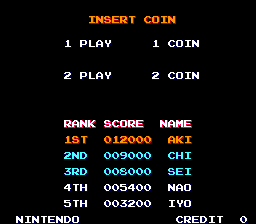
\includegraphics[width=0.25\textwidth]{../img/highscore}};
\end{tikzpicture}
\end{Slide}



\begin{Slide}{Algoritm-exempel: HIGHSCORE}
\Emph{Problem}: Uppdatera high-score i ett spel \\ \vspace{1em}

\Emph{Varför?} \pause Så att de som spelar uppmuntras att spela mer :) \\ \vspace{1em}

\Emph{Algoritm:}\pause
\begin{enumerate}
\item $points$ $\leftarrow$ poängen efter senaste spelet
\item $highscore$ $\leftarrow$ bästa resultatet innan senaste spelet
\item \Key{om} $points$ är större än $highscore$ 
\begin{enumerate}[ ~~]
\item  Skriv ''Försök igen!''
\end{enumerate}
\Key{annars}
\begin{enumerate}[ ~~]
\item  Skriv ''Grattis!''
\end{enumerate}
\end{enumerate}
\pause
\scriptsize \Alert{Hittar du buggen?}
\end{Slide}


\begin{Slide}{HIGHSCORE implementerad i Scala}
\begin{Code}
import scala.io.StdIn.readLine

object HighScore {
  def main(args: Array[String]): Unit = {
    val points = readLine("Hur mång poäng fick du?")
    val highscore = readLine("Vad var highscore före senaste spelet?")
    val msg = if (points > highscore) "GRATTIS!" else "Försök igen!"
    println(msg) 
  }
}
\end{Code}
\pause
Är det en bugg eller en feature att det står\\ \texttt{points > highscore} \\ och inte \\ \texttt{points >= highscore} \\ ?
% Buggen är att man inte får GRATTIS om poäng == highscore vilket är tråkigt :)
\end{Slide}



\begin{Slide}{Algoritmexempel: N-FAKULTET}
\begin{algorithm}[H]
 \SetKwInOut{Input}{Indata}\SetKwInOut{Output}{Resultat}

 \Input{heltalet $n$}
 \Output{utskrift av produkten av de första $n$ heltalen }
 ~\\
 $prod \leftarrow 1$ \\
 $i \leftarrow 2$  \\
 \While{$i \leq n$}{
  $prod \leftarrow prod * i$\\
  $i \leftarrow i + 1$
 }
 skriv ut $prod$
\end{algorithm}
\pause\vspace{1em}
\begin{itemize}\SlideFontSmall
\item Vad händer om $n$ är noll?
\item Vad händer om $n$ är ett?
\item Vad händer om $n$ är två?
\item Vad händer om $n$ är tre?
\end{itemize}
\end{Slide}

\begin{Slide}{Algoritmexempel: MIN}
\begin{algorithm}[H]
 \SetKwInOut{Input}{Indata}\SetKwInOut{Output}{Resultat}

 \Input{Array $args$ med strängar som alla innehåller heltal}
 \Output{utskrift av minsta heltalet }
 ~\\
 $min \leftarrow$ det största heltalet som kan uppkomma  \\
 $n \leftarrow $ antalet heltal \\
 $i \leftarrow 0$ \\
 \While{$i < n$}{
   $x \leftarrow args(i).toInt$ \\
   \If{( x < $min$)}{$min \leftarrow x$}
   $i \leftarrow i + 1$
 }
 skriv ut $min$
\end{algorithm}
\end{Slide}


\Subsection{Funktioner skapar struktur}

\begin{Slide}{Mall för funktionsdefinitioner}

\code{def} funktionsnamn(parameterdeklarationer): returtyp = block

\pause\vspace{0.5em}\Emph{Exempel}:

\begin{Code}[basicstyle=\ttfamily\fontsize{9}{11}\selectfont]
def öka(i: Int): Int = { i + 1 }
\end{Code}
\pause Om ett enda uttryck: behövs inga \code|{}|. Returtypen kan härledas.
\begin{Code}[basicstyle=\ttfamily\fontsize{9}{11}\selectfont]
def öka(i: Int) = i + 1  
\end{Code}
\pause Om flera parametrar, separera dem med kommatecken: 
\begin{Code}[basicstyle=\ttfamily\fontsize{9}{11}\selectfont]
def isHighscore(points: Int, high: Int): Boolean = {
  val highscore: Boolean = points > high
  if (highscore) println(":)") else print(":(")
  highscore
}
\end{Code}
\pause Ovan funktion har \Alert{sidoeffekten} att skriva ut en smiley.
\end{Slide}

\begin{Slide}{Bättre många små abstraktioner som gör en sak var}

\begin{Code}[basicstyle=\ttfamily\fontsize{8}{11}\selectfont]
def isHighscore(points: Int, high: Int): Boolean = points > high

def printSmiley(isHappy: Boolean): Unit = 
  if (isHappy) println(":)") else print(":(")
\end{Code}

\pause\vspace{2em}
\begin{REPLnonum}
  printSmiley(isHighscore(113,99))
\end{REPLnonum}

\pause\vspace{2em} \code{isHigscore} är en \Emph{äkta funktion} som alltid ger samma svar för samma inparametrar och saknar sidoeffekter.

\end{Slide}



\begin{Slide}{Vad är ett block?}

\begin{itemize}
\item Ett block \Emph{kapslar in} flera satser/uttryck och ser ''utifrån'' ut som en enda sats/uttryck.

\item Ett block skapas med hjälp av klammerparenteser (''krullparenteser'')

\item [] {\fontsize{14}{18}\selectfont \code|{ uttryck1; uttryck2; ... uttryckN }|}\\~

\pause

\item I Scala (till skillnad från många andra språk) har ett block ett \Emph{värde} och är alltså ett \Emph{uttryck}. 

\item Värdet ges av \Emph{sista uttrycket}.

\begin{REPLnonum}
scala> val x = { println(1 + 1); println(2 + 2); 3 + 3 } 
2
4
x: Int = 6
\end{REPLnonum}


\end{itemize}

\end{Slide}

\begin{Slide}{Block kan ha lokala variabler}\SlideFontSmall
Synlighetsregler etc
\end{Slide}


\begin{Slide}{Parameter och argument}\SlideFontSmall
\end{Slide}

\begin{Slide}{Procedurer}\SlideFontSmall
\begin{itemize}
\item En \Emph{procedur} är en funktion som \Alert{gör} något intressant, men som \Alert{inte} lämnar något intressant returvärde.
\item Exempel på befintlig procedur: \code{println("hej")}
\item Du \Emph{deklarerar egna procedurer} genom att ange \texttt{\Alert{Unit}} som returvärdestyp. Då ges värdet \texttt{\Alert{()}} som betyder ''inget''.
\end{itemize}
\begin{REPL}
scala> def hej(x: String): Unit = println(s"Hej på dej $x!")
hej: (x: String)Unit

scala> hej("Herr Gurka")
Hej på dej Herr Gurka!

scala> val x = hej("Fru Tomat")
Hej på dej Fru Tomat!
x: Unit = ()
\end{REPL}
\begin{itemize}
\item Det som \Alert{görs} kallas (sido)\Emph{effekt}. Ovan är utskriften själva effekten.
\item Funktioner kan också ha sidoeffekter. De kallas då \Alert{oäkta} funktioner.
\end{itemize}
\end{Slide}

\begin{Slide}{''Ingenting'' \emph{är} faktiskt någonting i Scala}
\begin{itemize}
\item I många språk (Java, C, C) är funktioner som saknar värden speciella.
 Java m.fl. har speciell syntax för procedurer med nyckelordet \jcode{void}, men \Alert{inte} Scala. 

\item I Scala är procedurer inte specialfall; de är vanliga funktioner som returnerar ett värde som \Emph{representerar} ingenting, nämligen () som är av typen Unit. 

\item På så sätt blir procedurer inget undantag utan följer vanlig syntax och semantik precis som för alla andra funktioner.

\item Detta är typiskt för Scala: generalisera koncepten och vi slipper besvärliga undantag! \\(Men vi måste förstå generaliseringen...)


\item [] {\SlideFontSmall 
\url{https://en.wikipedia.org/wiki/Void_type}
\url{https://en.wikipedia.org/wiki/Unit_type}
}

\end{itemize}

\end{Slide}

\begin{Slide}{Abstraktion: Problemlösning genom nedbrytning i enkla funktioner och procedurer som kombineras}\SlideFontSmall
\begin{itemize}
\item En av de allra viktigaste principerna inom programmering är \Emph{funktionell nedbrytning} där  \Emph{underprogram} i form av funktioner och procedurer skapas för att bli byggstenar som kombineras till mer avancerade funktioner och procedurer.

\item Genom de namn som definieras skapas \Emph{återanvändbara abstraktioner} som kapslar in det funktionen gör. 

\item Problemet blir med bra byggblock lättare att lösa.

\item Abstraktioner som beräknar eller gör \Emph{en enda, väldefinierad sak} är enklare att använda, jämfört med de som gör många, helt olika saker.

\item Abstraktioner med \Emph{välgenomtänkta namn} är enklare att använda, jämfört med kryptiska eller missvisande namn.
\end{itemize}

\end{Slide}

\begin{Slide}{Exempel på funktionell nedbrytning}
$<<$kvadrat, stapel, rutnät i kojo$>>$ 
\end{Slide}


\Subsection{Kodfilernas katalogstruktur}

\begin{Slide}{Paket}
$<<$paket skapar katalogstruktur för kodfiler$>>$ 
\end{Slide}

\begin{Slide}{Jar-filer}
$<<$liknar zip-filer; packar ihop bytekod i en enda fil för enkel distribution$>>$ 
\end{Slide}

\subsection{Att göra denna vecka}


%%%
\frame{\frametitle{Att göra i Vecka \vecka: Förstå grundläggande kodstrukturer}
\begin{enumerate}
\item Laborationer är \Alert{obligatoriska}.\\ Ev. sjukdom måste anmälas \Alert{före} via mejl till kursansvarig!
\item Gör övning \texttt{programs}
\item OBS! Ingen lab denna vecka w02. Använd tiden att komma ikapp om du ligger efter!
\item Träffas i samarbetsgrupper och hjälp varandra att förstå.
\item Vi har nosat på flera koncept som vi kommer tillbaka till senare: du måste inte fatta alla detaljer redan nu.
\item Om ni inte redan gjort det: Gör klart \href{https://github.com/bjornregnell/lth-eda016-2015/tree/master/assignments}{samarbetskontrakt} och visa för handledare på resurstid.
\item \Alert{Koda på resurstiderna} och få hjälp och tips! 
\end{enumerate}
}








